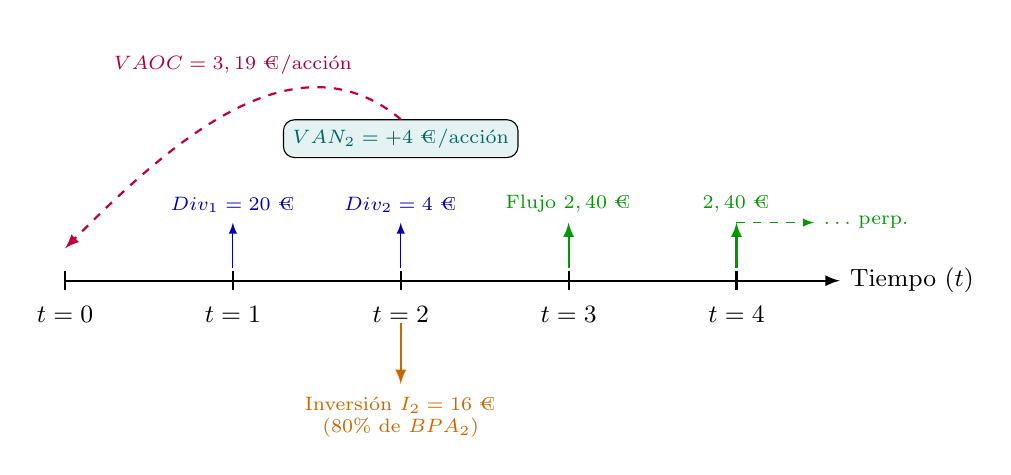
\begin{tikzpicture}[scale=0.82, >=latex]
  % Eje temporal
  \draw[->, thick] (0,0) -- (12.0,0) node[right, font=\small] {Tiempo ($t$)};

  % Marcas temporales
  \foreach \t/\x in {0/0, 1/2.6, 2/5.2, 3/7.8, 4/10.4} {
    \draw[thick] (\x,0.15) -- (\x,-0.15) node[below=2pt, font=\small] {$t=\t$};
  }

  % En t=1: Dividendo normal (una sola línea para máxima holgura vertical)
  \draw[->, blue!70!black] (2.6, 0.2) -- (2.6, 0.9) 
    node[above, font=\scriptsize] {$Div_1 = 20$ €};

  % En t=2: Dividendo corriente
  \draw[->, blue!70!black] (5.2, 0.2) -- (5.2, 0.9) 
    node[above, font=\scriptsize] {$Div_2 = 4$ €};

  % Inversión en t=2 hacia abajo (inicia bajo el rótulo t=2)
  \draw[->, orange!80!black, thick] (5.2, -0.65) -- (5.2, -1.6) 
    node[below=1pt, font=\scriptsize, align=center] {Inversión $I_2 = 16$ €\\($80\%$ de $BPA_2$)};

  % En t=3 en adelante: Renta perpetua generada
  \draw[->, green!60!black, thick] (7.8, 0.2) -- (7.8, 0.9) 
    node[above, font=\scriptsize] {Flujo $2,40$ €};
  \draw[->, green!60!black, thick] (10.4, 0.2) -- (10.4, 0.9) 
    node[above, font=\scriptsize] {$2,40$ €};
  \draw[->, green!60!black, dashed] (10.4, 0.9) -- (11.6, 0.9) node[right, font=\scriptsize] {$\dots$ perp.};

  % Cuadro VAN en t=2 (bien elevado para no tocar Div2)
  \node[draw, rounded corners, fill=teal!10, text=teal!80!black, font=\scriptsize, align=center] (van2) at (5.2, 2.2)
    {$VAN_2 = +4$ €/acción};

  % Descuento a t=0 (arco holgado que vuela alto sobre Div1)
  \draw[->, purple, thick, dashed] (5.2, 2.5) to[out=140, in=45] (0, 0.5);
  \node[above, font=\scriptsize, text=purple!90!black, fill=white, inner sep=2pt] at (2.6, 3.1)
    {$VAOC = 3,19$ €/acción};
\end{tikzpicture}
